\documentclass{article}
\usepackage{graphicx}
\usepackage{amsmath}
\usepackage{gensymb}

\author{Timothy Boose\\Reed Fowler\\Justin Joy\\Dylan Orozco\bigskip\\Physics 188}
\date{\today}
\title{Lab 7 Report - Group 7}

\begin{document}
\maketitle

\section{Goal}

The goal of this lab was to do the following:

\begin{itemize}
    \item e
\end{itemize}

\section{Skills Learned}

We learned the following skills during this exercise:

\begin{itemize}
    \item e
\end{itemize}

\section{Data Collected}

The following data was collected:

\begin{itemize}
    \item e
\end{itemize}

The following data was provided and used in our analysis:

\begin{itemize}
    \item e
\end{itemize}

\section{Analysis of Data}

\section{Figures}
\begin{center}
    \begin{figure}[h!bt]
        \caption{
            e
            \smallskip
        }
        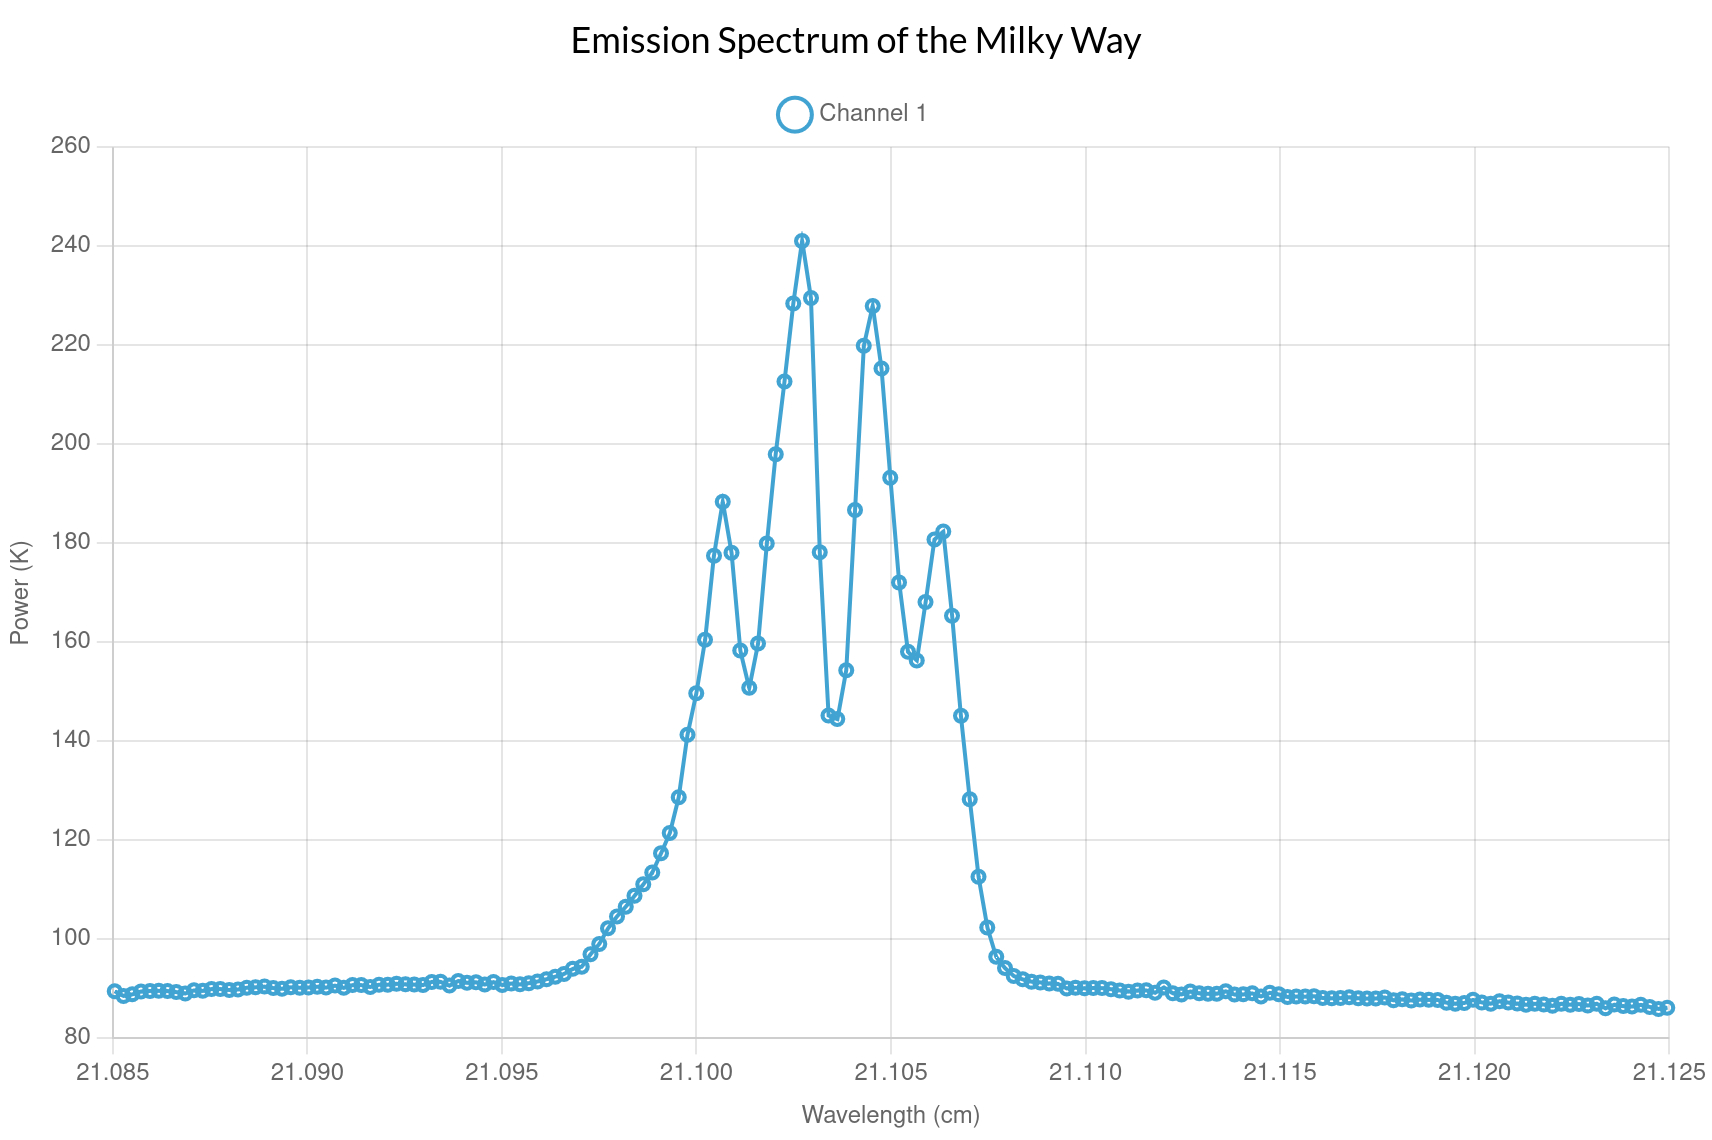
\includegraphics[scale=0.1]{emission-graph-lab9.jpg}
        \centering
    \end{figure}
    \begin{figure}[h!bt]
        \caption{
            e
            \smallskip
        }
        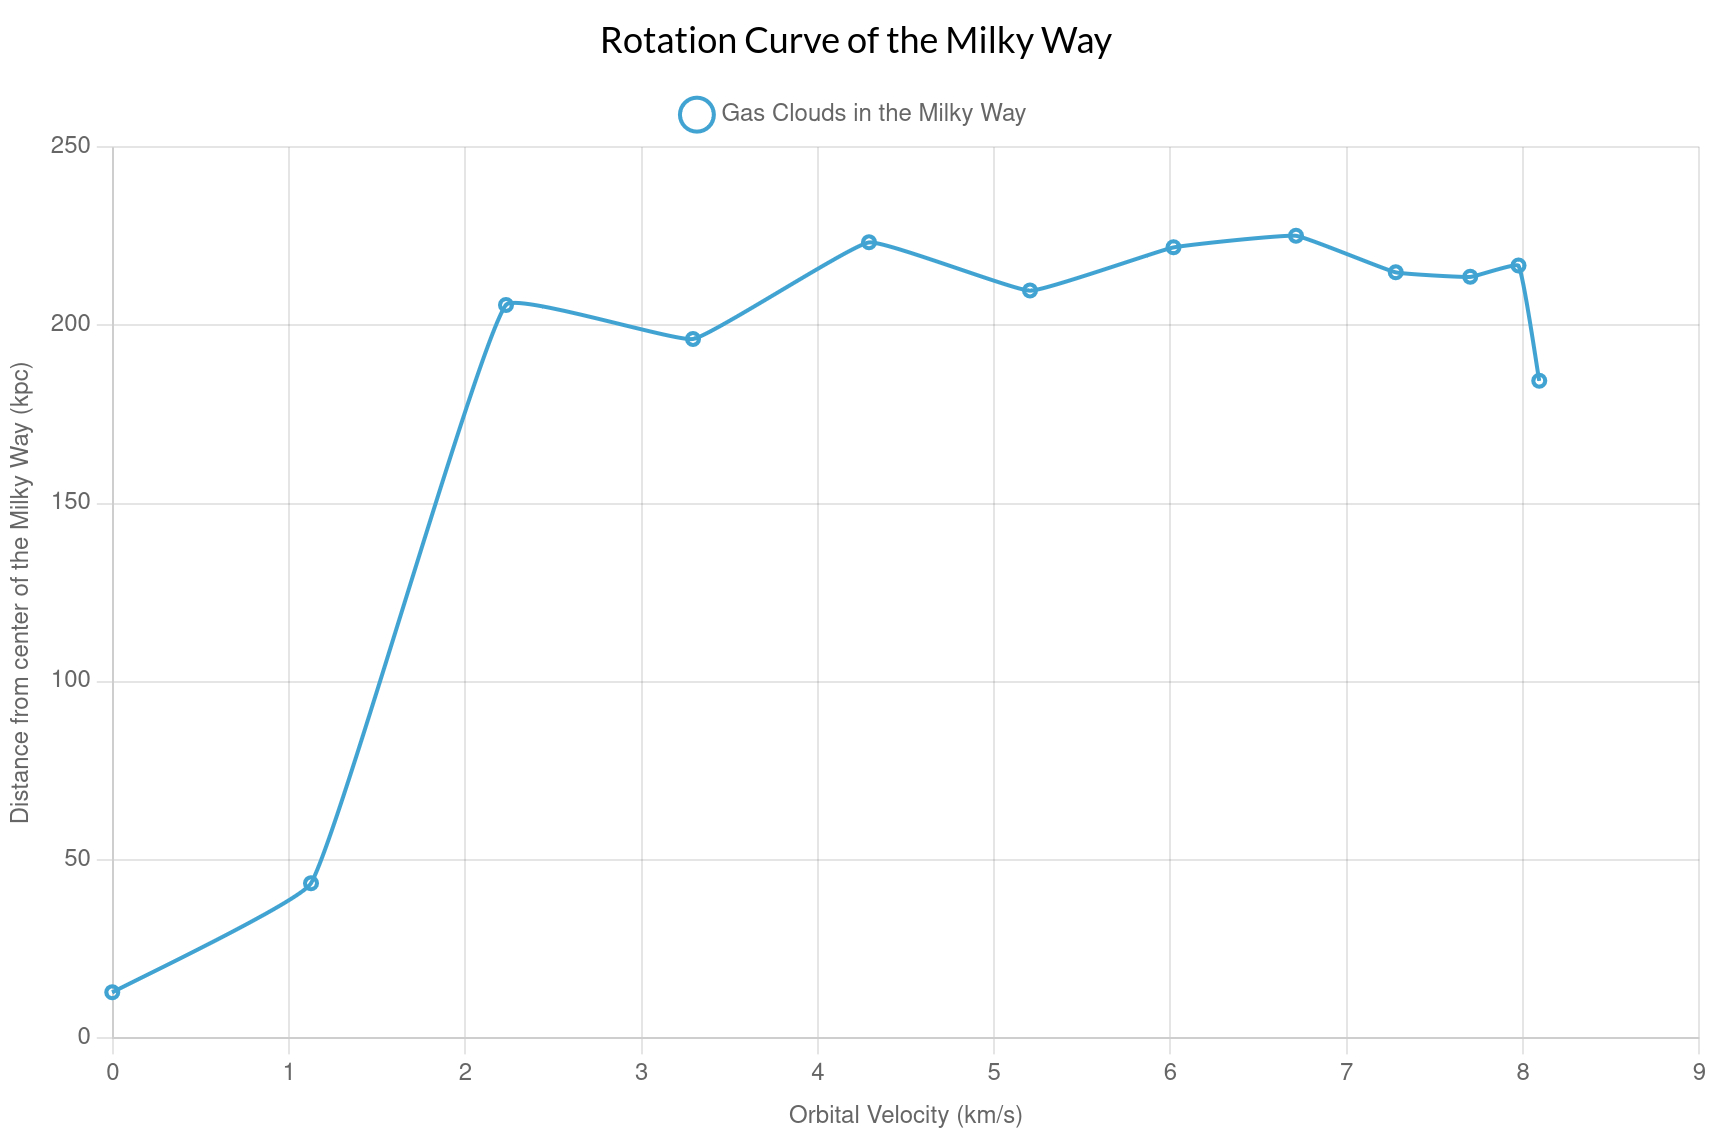
\includegraphics[scale=0.1]{rotation-curve-lab9.jpg}
        \centering
    \end{figure}
    \begin{figure}[h!bt]
        \caption{
            e
            \smallskip
        }
        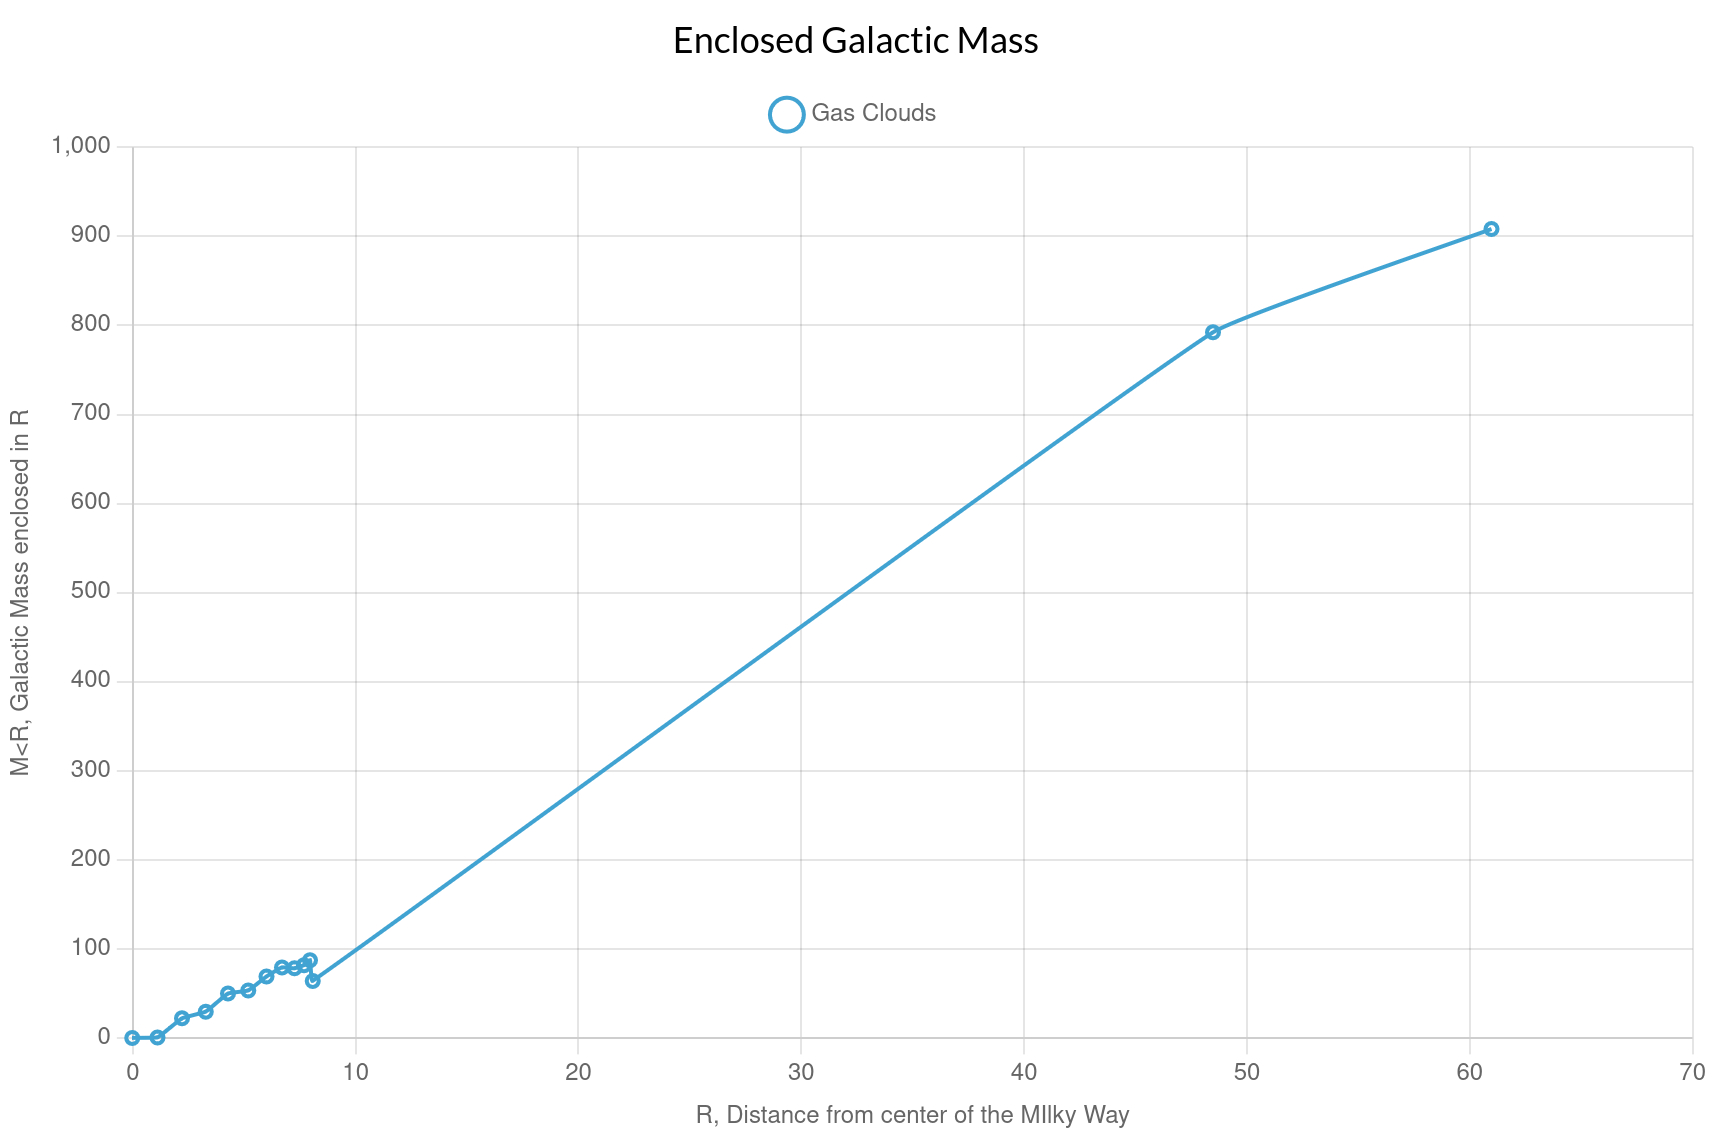
\includegraphics[scale=0.1]{distance-enclosed-mass.jpg}
        \centering
    \end{figure}
\end{center}

\section{Conclusion}



\section{Limitations}



\subsection{Errors}



\subsection{Impact of Errors}



\end{document}